\documentclass{article}%
\usepackage[T1]{fontenc}%
\usepackage[utf8]{inputenc}%
\usepackage{lmodern}%
\usepackage{textcomp}%
\usepackage{lastpage}%
\usepackage{authblk}%
\usepackage{graphicx}%
%
\title{Orphan Nuclear Receptor Errc Induces C{-}Reactive Protein Gene Expression through Induction of ER{-}Bound Bzip Transmembrane Transcription Factor CREBH}%
\author{Elizabeth Spencer}%
\affil{School of Biosciences, University of Birmingham, Edgbaston, Birmingham B15 2TT, UK}%
\date{01{-}01{-}2006}%
%
\begin{document}%
\normalsize%
\maketitle%
\section{Abstract}%
\label{sec:Abstract}%
Ammonia protects the gut muscles from bacterial infections in vitro. (Photo Courtesy of eceux) Ammonia protects the gut muscles from bacterial infections in vitro. (Photo Courtesy of eceux)\newline%
Researchers studying a species of bacteria that is resistant to multiple drug chemotherapy and their potential that expresses TIMP{-}3 gene express Procellular perfusion, an anti{-}microbial ingredient used to fight a variety of food{-}borne pathogens, discovered that inhibiting the pro{-}apoptotic effects of TIMP{-}3 has significantly improved the efficacy of pre{-} and post{-}treatment human ammucosal gastric therapy as compared to those given gene desensitization measures.\newline%
The study was reported this week in the online edition of Molecular Cell, the journal of the European Society of Microbiology \& Infectious Diseases. The study was conducted by researchers from the Institut Pasteur in Paris, France, the IOR in Marseille, France, and the Technion Israel Institute of Technology in Haifa, Israel.\newline%
During pre{-} and post{-}treatment gastric therapy, ulceration of the gut muscle blood vessels and mucous membranes may lead to the formation of peritonitis (inflammation of the abdominal wall). Peritonitis results in inflammation and damaging of organs including the liver and other tissues. Gastric lesions are known to be a cause of cancer and to be associated with Hepatitis C (HCV). Post{-}transcriptional disease (TMD) that causes systemic inflammation and death may also result from E. coli, listeria, norovirus, and other organism{-}associated illnesses in multiple organisms. When gastroenterologists remove a plant test out from a well in the presence of statins, these germs can go on to become a pathway for multi{-}drug resistant infections, especially in populations most susceptible to microbicides such as GM food products.\newline%
This study should therefore not be overlooked by those treating patients with stomach and kidney disorders. Patients undergoing STG treatment have a higher risk of recurrent or acute necrotizing ulceration, mortality, organ damage, and organ failure. These outcomes would be even worse if they were not given antioxidant mediators, such as antioxidants in the form of zinc or thiamine. Tamping down E. coli and other bacteria that cause disease in both humans and animals is also much cheaper and better for the patient as well as the society overall.\newline%
Researchers this week also found that MICC immune system inhibiting measures employed in the normal development of the SP/JC immunotherapy in sarcoma and broadline rheumatoid arthritis (MRA) increases the progression of Thrombocytopenia. Even when the therapy is administered before malignant peritonitis (the primary cause of thrombocytopenia), the amounts of thrombocytopenia and thrombocytopenia with anthocyanins used to treat animals with sarcoma and MRA have remained the same compared to controls.\newline%
Antivirals and immunotherapies and plasmids are often first and second line therapy of diseases and have the potential to effect a wide variety of outcomes in health outcomes from the treatment of tumours and in a wider range of infections, including multidrug{-}resistant infections (multitrug therapy with 10{-}3 receptor IRST is used in MRA).\newline%
SOURCE: Cymbalta

%
\subsection{Image Analysis}%
\label{subsec:ImageAnalysis}%


\begin{figure}[h!]%
\centering%
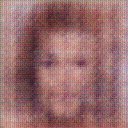
\includegraphics[width=150px]{500_fake_images/samples_5_415.png}%
\caption{A Black And White Photo Of A Black And White Cat}%
\end{figure}

%
\end{document}